\chapter{Planification du projet}

\section*{Introduction}
Ce chapitre commence par la spécification des besoins, en présentant les besoins fonctionnels et non fonctionnels. Ensuite, il aborde la gestion du projet avec Scrum, en présentant l'équipe Scrum, le backlog du produit et la planification de la release. Enfin, nous examinons l'environnement de développement, l'architecture et les patrons de conception adaptés.

\section{Spécification des besoins}

Notre projet vise à développer une plateforme de marketplace d'API « Infinity API », permettant aux développeurs et aux entreprises d'intégrer et de consommer facilement des API de manière simplifiée. //
Afin d'atteindre cet objectif, nous exposons les exigences fonctionnelles et non fonctionnelles de notre plateforme.

    \subsection{Les besoins fonctionnels } 
    Les besoins fonctionnels de notre projet se résument comme suit :
    \begin{itemize}
        \item  \textbf{Gestion des API}
        \begin{itemize}
            \item Ajout d’une API avec la documentation Swagger, qui regroupe ainsi les endpoints, les descriptions des requêtes et des réponses.
            \item Consultation, modification et suppression d'une API par un développeur. 
        \end{itemize}
        \item \textbf{Gestion de la tarification des API}
        \begin{itemize}
            \item Création, modification et suppression de plans de tarification pour une API. Un plan de tarification est composé du nom du plan, du nombre de requêtes, de la durée et du prix.
            \item Consultation des plans de tarification disponibles pour une API. 
        \end{itemize}
        \item \textbf{Catalogue d’API}
        \begin{itemize}
            \item Consultation de la liste des API par un utilisateur. 
            \item Filtrage des APIs selon différents critères. 
            \item Consultation des détails de chaque API. 
        \end{itemize}
        \item \textbf{Gestion de la souscription à une API}
        \begin{itemize}
            \item Souscription à une API après avoir choisi le plan de tarification qui convient pour un plan de tarification payant, la souscription engendre une opération de paiement. 
            \item Consultation de la liste des souscriptions.  
            \item Annulation d’une souscription. 
            \item Consultation de l'historique des souscriptions.
            \item Mise à niveau de la souscription pour obtenir un quota de requêtes plus élevé et une durée de validité étendue.
            \item Consultation de l'historique des payements.
        \end{itemize}
        \item \textbf{Consommation et test des API}
        \begin{itemize}
            \item Consommation d’une API, qui consiste à utiliser les endpoints pour effectuer des requêtes et récupérer les données nécessaires.
            \item Test des API et leur consommation sur la plateforme « Infinity API ».          
        \end{itemize}
        \item \textbf{Gestion des transactions}
        \begin{itemize}
            \item Consultation du montant disponible sur le compte d’un développeur gagner de la plateforme.
            \item Vérification des transactions effectuées sur l’API fournier par un développeur.
            \item Demande d’un prélèvement du solde disponible sur le compte.
            \item Gestion des demandes de prélèvement par l'administrateur.    
        \end{itemize}
        \item \textbf{Dashboard Administrateur}
        \begin{itemize}
            \item Consultation de la liste des développeurs inscrits sur la plateforme.
            \item Blocage et déblocage d’un compte développeur.   
        \end{itemize}
        \item \textbf{Gestion des catégories} \\
         Ajout, modification, suppression et consultation de catégories.
         \item \textbf{Gestion des comptes utilisateur }
         \begin{itemize}
             \item Inscription d'un nouveau développeur.
             \item Consultation, modification d’un profil utilisateur.   
             \item Suppression d'un profil développeur.
         \end{itemize}
         \item \textbf{Gestion des signalements de problèmes}
         \begin{itemize}
             \item Signalement d’un problème lié à une API.
             \item Consultation des signalements par l’administrateur et par le développeur qui a fourni l’API.  
         \end{itemize}
         \item \textbf{Gestion des feedbacks}
         \begin{itemize}
             \item Création, modification, et suppression d’un commentaire relatif à une API.
             \item Consultation des commentaires laissés par les développeurs. 
         \end{itemize}
         \item \textbf{Suivi et statistiques }
         \begin{itemize}
             \item Suivi des payements et des statistiques liées à l’utilisation de la plateforme.
             \item Suivi des statistiques de performance et d'état des APIs.
             \item Suivi des statistiques de paiement des APIs.
         \end{itemize}
         \item \textbf{Système de notification  } \\
         La marketplace doit fournir des notifications suite aux différentes opérations effectuées sur la plateforme.
    \end{itemize}        
    % Une deuxième sous section
    \subsection{Les besoins non fonctionnels }
    Les besoins non fonctionnels de notre projet se résument comme suit : 
    \begin{itemize}
        \item \textbf{Sécurité des données }
        \begin{itemize}
            \item Authentification des utilisateurs.
            \item o	Utilisation de mécanismes de sécurité pour protéger les données des utilisateurs.
        \end{itemize}
        \item \textbf{Ergonomie de l'interface }\\
        La navigation intuitive et claire entre les différentes interfaces de l'application.
        \item \textbf{Fiabilité  }\\
        Minimiser les erreurs de serveur pour garantir une expérience utilisateur stable et fiable.
        \item \textbf{Documentation des API avec Swagger  }\\
        Utilisation de Swagger pour créer une documentation détaillée des API ajoutées à la plateforme, facilitant ainsi l'intégration et l'utilisation par les développeurs tiers.
        \item \textbf{Intégration de services de paiement en ligne }\\
        Intégration de services comme Stripe et PayPal pour permettre des transactions sécurisées lors de la souscription aux plans de tarification payants et des prélèvements de solde.
    \end{itemize}        

% Une deuxième section Pilotage du projet avec Scrum 
\section{Pilotage du projet avec Scrum }
Dans cette partie, nous allons aborder la présentation de l'équipe Scrum ainsi que le backlog du produit et pour finir, la planification de la release.
    \subsection{Equipe et rôles  } 
    Avant de présenter le product backlog, il est important d'introduire l'équipe de travail :
    \begin{itemize}
        \item \textbf{Le Product Owner }:M.Akram ANAYA :Chef projet de l’équipe de développement 
        \item \textbf{Le Scrum Master }: M.Ahmed GHIZWENI : Chef de produit
        \item \textbf{Les développeurs  }: Yassine LASSOUED et Ayoub SHILI
    \end{itemize} 
    \subsection{Le backlog du produit  } 
    Nous avons utilisé une échelle basée sur la suite de Fibonacci. Les valeurs attribuées sont les suivantes  : 1 pour "Très facile", 2 pour "Facile", 3 pour "Assez simple", 5 pour "Moyen", 8 pour "Assez compliqué", 13 pour "Compliqué" et 20 pour "Très compliqué". Dans le cas de notre marketPlace ,les utilisateurs sont : \\
    \begin{itemize}
        \item \textbf{Visiteur }:c’est un internaute qui n'a pas encore été authentifié.
        \item \textbf{Développeur  }: qui est inscrit sur notre plateforme, il peut jouer le rôle de fournisseur ou de consommateur d’API
        \item \textbf{Administrateur }: qui gère la plateforme.
    \end{itemize} 

    \begin{longtable}[c]{
        |p{.10\textwidth}
        |p{.20\textwidth}
        |p{.10\textwidth}
        |p{.30\textwidth}
        |p{.10\textwidth}
        |p{.05\textwidth}
        |p{.05\textwidth}|
    }
        \caption{Tableau long}
        \label{tab:myfirstlongtable}\\
        \hline
        \textbf{US ID} & \textbf{Thème} & \textbf{En Tant que} & \textbf{User Story} & \textbf{Valeur Business} & \textbf{Effort} & \textbf{Priorité} \\
        \hline 
        \endfirsthead
        \multicolumn{7}{c}%
        {{\bfseries \tablename\ \thetable{} -- suite de la page précédente}} \\
        \hline 
        \textbf{US ID} & \textbf{Thème} & \textbf{En Tant que} & \textbf{User Story} & \textbf{Valeur Business} & \textbf{Effort} & \textbf{Priorité} \\
        \hline 
        \endhead
        \hline \multicolumn{7}{|r|}{{\bfseries Suite à la page suivante}} \\ \hline
        \endfoot
        \hline
        \endlastfoot
        
        1 & Création du compte Utilisateur & Visiteur & Je souhaite pouvoir m'inscrire pour créer un compte. & Haute & 5 & Haute \\
        \hline
        2 & Authentification & Développeur ou Administrateur & Je souhaite pouvoir m'authentifier pour accéder à mon compte. & Haute & 13 & Haute \\
        \hline
        3 & Gestion des catégories & Administrateur & Je veux créer une nouvelle catégorie en spécifiant son nom, sa description et d'autres informations pertinentes. & Haute & 2 & Haute \\
        \hline
        4 & & Administrateur & Je veux modifier les détails d'une catégorie existante. & Haute & 2 & Haute \\
        \hline
        5 & & Administrateur & Je veux supprimer une catégorie. & Haute & 1 & Haute \\
        \hline
        6 & & Administrateur & Je veux consulter la liste des catégories existantes sur la plateforme. & Haute & 2 & Haute \\
        \hline
        7 & Gestion des APIs & Développeur & Je veux pouvoir ajouter une nouvelle API pour fournir une API aux autres utilisateurs. & Haute & 20 & Haute \\
        \hline
        8 & & Développeur & Je veux consulter la liste de mes APIs pour visualiser rapidement toutes les APIs que j'ai créées. & Haute & 5 & Haute \\
        \hline
        9 & & Développeur & Je veux pouvoir modifier les informations de mon API pour mettre à jour les informations. & Haute & 5 & Haute \\
        \hline
        10 & & Développeur & Je veux pouvoir supprimer mon API car elle n'existe plus ou contient beaucoup de signalments d'erreurs. & Haute & 2 & Haute \\
        \hline
        11 & Consultation, filtrage et recherche sur les APIs & Utilisateur & Je veux pouvoir consulter la liste des APIs pour pouvoir chercher l’API qui répond à mes besoins. & Haute & 5 & Haute \\
        \hline
        12 & & Utilisateur & Je veux pouvoir consulter les détails d'une API pour découvrir ses fonctionnalités. & Haute & 8 & Haute \\
        \hline
        13 & & Utilisateur & Je veux pouvoir rechercher une API par son nom pour la trouver rapidement et facilement. & Haute & 2 & Haute \\
        \hline
        14 & & Utilisateur & Je veux pouvoir faire un filtrage avancé sur les APIs pour trouver celles qui correspondent le mieux à mes besoins. & Haute & 5 & Haute \\
        \hline
        15 & Gestion du compte Utilisateur & Développeur ou Administrateur & Je veux pouvoir consulter mon profil pour vérifier mes informations personnelles. & Haute & 3 & Haute \\
        \hline
        16 & & Développeur ou Administrateur & Je veux pouvoir modifier mon profil pour mettre à jour mes informations. & Haute & 5 & Haute \\
        \hline
        17 & & Développeur & Je veux pouvoir supprimer mon compte pour me désinscrire de la plateforme. & Haute & 2 & Haute \\
        \hline
        18 & Gestion de la tarification & Développeur & Je veux pouvoir créer des plans de tarification pour mon API pour proposer différents niveaux d'accès à mon API et générer des revenus. & Moyenne & 8 & Haute \\
        \hline
        19 & & Développeur & Je veux pouvoir consulter les plans de tarification pour suivre les options disponibles pour mes APIs. & Moyenne & 3 & Haute \\
        \hline
        20 & & Développeur & Je veux pouvoir modifier des plans de tarification pour mon API pour pouvoir mettre à jour les prix et les limites d'utilisation. & Moyenne & 5 & Haute \\
        \hline
        21 & & Développeur & Je veux pouvoir supprimer un plan de tarification pour mon API si la tarification n'est plus nécessaire. & Moyenne & 2 & Haute \\
        \hline
        22 & & Utilisateur & Je veux pouvoir consulter les plans de tarification pour une API afin de choisir celui qui correspond le mieux à mes besoins et à mon budget. & Moyenne & 3 & Haute \\
        \hline
        23 & Souscription & Développeur & Je veux pouvoir souscrire à une API pour accéder aux fonctionnalités qu'elle propose. & Moyenne & 20 & Haute \\
        \hline
        24 & & Développeur & Je veux pouvoir consulter la liste de mes souscriptions pour suivre mes souscriptions. & Moyenne & 2 & Haute \\
        \hline
        25 & & Développeur & Je veux pouvoir effectuer une mise à niveau de ma souscription d'API. & Moyenne & 8 & Haute \\
        \hline
        26 & & Développeur & Je veux pouvoir annuler une souscription. & Moyenne & 3 & Haute \\
        \hline
        27 & Consommation et test d'une API & Développeur & Je veux pouvoir consommer une API et l'intégrer dans mon projet afin d'utiliser ses fonctionnalités. & Moyenne & 13 & Haute \\
        \hline
        28 & & Développeur & Je veux pouvoir tester l'API sur la plateforme pour savoir si elle fonctionne correctement et qu'elle répond aux besoins des développeurs. & Moyenne & 20 & Haute \\
        \hline
        29 & Dashboard Administrateur & Administrateur & Je veux pouvoir consulter la liste des développeurs et suivre leurs activités. & Moyenne & 3 & Moyenne \\
        \hline
        30 & & Administrateur & Je veux pouvoir rechercher un utilisateur. & Moyenne & 2 & Moyenne \\
        \hline
        31 & & Administrateur & Je veux pouvoir consulter les détails d'un développeur pour comprendre son activité et ses interactions avec la plateforme. & Moyenne & 8 & Moyenne \\
        \hline
        32 & & Administrateur & Je veux pouvoir bloquer/débloquer un compte développeur pour contrôler tout comportement abusif ou non autorisé. & Moyenne & 3 & Moyenne \\
        \hline
        33 & Gestion des transactions & Développeur & Je veux pouvoir consulter le montant disponible sur mon compte afin de suivre mes revenus générés par la vente d'API sur la plateforme. & Moyenne & 3 & Moyenne \\
        \hline
        34 & & Développeur & Je veux pouvoir vérifier les transactions effectuées via mon API afin de tracer l'origine de mes revenus. & Moyenne & 3 & Moyenne \\
        \hline
        35 & & Développeur & Je veux pouvoir effectuer une demande de prélèvement du solde disponible sur le compte. & Moyenne & 8 & Moyenne \\
        \hline
        36 & & Administrateur & Je veux pouvoir gérer les demandes de prélèvement en les acceptant ou en les refusant. & Moyenne & 5 & Haute \\
        \hline
        37 & Dashboards de Statistiques & Développeur & Je veux pouvoir suivre les statistiques de performance de mon API pour surveiller son utilisation et sa qualité de service. & Faible & 13 & Moyenne \\
        \hline
        38 & & Développeur & Je veux pouvoir suivre les statistiques d'utilisation de mon API (nombre de requêtes, nombre de développeurs, etc.) pour suivre l'utilisation de mon API. & Faible & 20 & Moyenne \\
        \hline
        39 & & Administrateur & Je veux pouvoir suivre les statistiques de performance des API pour surveiller la qualité de service globale de la plateforme. & Faible & 13 & Moyenne \\
        \hline
        40 & & Administrateur & Je veux pouvoir suivre les statistiques des paiements sur la plateforme pour surveiller les revenus de la plateforme. & Faible & 13 & Moyenne \\
        \hline
        41 & Gestion des signalements & Développeur & Je veux pouvoir signaler un problème pour obtenir une assistance ou signaler des problèmes de fonctionnement. & Faible & 5 & Moyenne \\
        \hline
        42 & & Développeur & Je veux pouvoir consulter mes signalements d'erreurs. & Faible & 3 & Moyenne \\
        \hline
        43 & & Administrateur & Je veux pouvoir consulter les signalements d'erreur pour suivre les problèmes identifiés par les développeurs. & Faible & 3 & Faible \\
        \hline
        44 & Gérer les feedbacks & Développeur & Je veux pouvoir ajouter un commentaire à une API pour partager mon avis sur l'API. & Faible & 3 & Faible \\
        \hline
        45 & & Développeur & Je veux pouvoir consulter les commentaires laissés par les développeurs d'une API afin de connaître leur opinion sur celle-ci. & Faible & 2 & Faible \\
        \hline
        46 & & Développeur & Je veux pouvoir modifier mon commentaire si je souhaite les rectifier. & Faible & 2 & Faible \\
        \hline
        47 & & Développeur & Je veux pouvoir supprimer mon commentaire si je souhaite le retirer de la plateforme. & Faible & 2 & Faible \\
        \hline
        48 & Système de notification & Développeur ou Administrateur & Je veux pouvoir consulter les notifications. & Faible & 8 & Faible \\
        \hline
    
    \end{longtable}

    \textbf{Utilisateur } ayant pour rôle visiteur, développeur ou administrateur
    \subsection{Planification de la release } 
    La planification de la release est une pratique agile consistant à diviser le travail en itérations courtes. Nous avons découpé notre release en 3 sprints de 4 semaines, comme l’illustré le tableau suivant.

    \documentclass{article}
    \usepackage{longtable}

    \begin{document}

    \begin{longtable}[c]{
        |p{.15\textwidth}
        |p{.25\textwidth}
        |p{.25\textwidth}
        |p{.25\textwidth}|
    }
        \caption{Planning des Sprints}
        \label{tab:sprintplanning}\\
        \hline
        \textbf{} & \textbf{Sprint 1} & \textbf{Sprint 2} & \textbf{Sprint 3} \\
        \hline
        \endfirsthead
        \multicolumn{4}{c}%
        {{\bfseries \tablename\ \thetable{} -- suite de la page précédente}} \\
        \hline
        \textbf{} & \textbf{Sprint 1} & \textbf{Sprint 2} & \textbf{Sprint 3} \\
        \hline
        \endhead
        \hline \multicolumn{4}{|r|}{{\bfseries Suite à la page suivante}} \\ \hline
        \endfoot
        \hline
        \endlastfoot

        \textbf{Date début et fin} & Due 04-03-2024 au 29-03-2024 & Due 01-04-2024 au 26-04-2024 & Due 29-04-2024 au 24-05-2024 \\
        \hline
        \textbf{Objectif} & 
        L'objectif du sprint 1 est de fournir aux utilisateurs la possibilité de créer leur compte utilisateur, ainsi que de créer une API et de la rendre disponible sur la marketplace et de gérer leur profil. &
        L'objectif du sprint 2 est de permettre aux utilisateurs d'intégrer la tarification dans leur API, de gérer leurs souscriptions, de consommer les APIs disponibles dans le catalogue et de développer un tableau de bord administrateur pour gérer les utilisateurs. &
        L'objectif du sprint 3 est de développer un tableau de bord permettant aux utilisateurs d'analyser l'utilisation de leurs APIs via des statistiques et de gérer leurs transactions. Il vise également à permettre aux administrateurs de suivre les statistiques des APIs et des paiements. De plus, il inclut la mise en place d'un système de notifications pour la gestion des signalements et des messages ainsi que la gestion des feedbacks. \\
        \hline
        \textbf{Les User Stories} & 1 jusqu’à 17 & 19 jusqu’à 32 & 33 jusqu’à 48 \\
        \hline
        \textbf{Estimation} & 87 & 103 & 106 \\
        \hline

    \end{longtable}

    \end{document}

\section{Environnement de travail}
    Cette partie présente spécifiquement l'environnement matériel et logiciel utilisés pour mettre en œuvre notre application.
    \subsection{Environnement matériel } 
    Les matériels utilisés pour notre projet se résument comme suit :
    \begin{longtable}[c]{
        |p{.20\textwidth}
        |p{.25\textwidth}
        |p{.20\textwidth}
        |p{.25\textwidth}|
    }
        \caption{Spécifications des Ordinateurs}
        \label{tab:computerspecs}\\
        \hline
        \textbf{Nom de l'ordinateur} & \textbf{Processeur} & \textbf{RAM} & \textbf{Disque Dur} & \textbf{Système d'exploitation} \\
        \hline
        \endfirsthead
        \multicolumn{4}{c}%
        {{\bfseries \tablename\ \thetable{} -- suite de la page précédente}} \\
        \hline
        \textbf{Nom de l'ordinateur} & \textbf{Processeur} & \textbf{RAM} & \textbf{Disque Dur} & \textbf{Système d'exploitation} \\
        \hline
        \endhead
        \hline \multicolumn{4}{|r|}{{\bfseries Suite à la page suivante}} \\ \hline
        \endfoot
        \hline
        \endlastfoot
        
        Yassine-MSI & 10th Gen Intel® Core™ i7-1015G4 @ 3.00GHz × 4 & 24 Go & 1 To HDD + 512 Go SSD & Windows 11 \\
        \hline
        Asus-PC & 11th Gen Intel(R) Core(TM) i5-11400H @ 2.70GHz   2.69 GHz & 16 Go & 1 To SSD & Windows 11 \\
        \hline
    \end{longtable}
    \subsection{Environnement logiciel  } 
    Les logiciels utilisés pour notre projet se résument comme suit :


    \begin{longtable}[c]{
        |p{.15\textwidth}
        |p{.75\textwidth}|
    }
        \caption{Description des Logiciels, Bibliothèques et Frameworks}
        \label{tab:softwaredesc}\\
        \hline
        \textbf{Logo} & \textbf{Description} \\
        \hline
        \endfirsthead
        \multicolumn{2}{c}%
        {{\bfseries \tablename\ \thetable{} -- suite de la page précédente}} \\
        \hline
        \textbf{Logo} & \textbf{Description} \\
        \hline
        \endhead
        \hline \multicolumn{2}{|r|}{{\bfseries Suite à la page suivante}} \\ \hline
        \endfoot
        \hline
        \endlastfoot
        
        
\includegraphics[width=0.1\textwidth]{angular_logo.png} & Angular 17 : est un Framework côté client (front end) à code source ouvert basé sur TypeScript dirigé par l’équipe du projet Angular de Google qui permet de construire des applications web dynamiques. \\
        \hline
        
\includegraphics[width=0.1\textwidth]{html_logo.png} & HTML (pour HyperText Markup Language) : est le langage utilisé pour structurer une page web et son contenu. \\
        \hline
        
\includegraphics[width=0.1\textwidth]{css_logo.png} & CSS (Cascading Style Sheets) : est un langage de feuille de style utilisé pour la mise en forme des pages HTML. \\
        \hline
        
\includegraphics[width=0.1\textwidth]{tailwind_logo.png} & Tailwind UI : est une collection de superbes composants d'interface utilisateur entièrement réactifs. Il propose des centaines d'exemples prêts à l'emploi. \\
        \hline
        
\includegraphics[width=0.1\textwidth]{swagger_logo.png} & Swagger UI permet de visualiser et d'interagir avec les ressources de l'API sans qu'aucune logique de mise en œuvre ne soit en place. Il est automatiquement généré à partir de votre spécification OpenAPI avec la documentation visuelle facilitant la mise en œuvre back-end et la consommation côté client. \\
        \hline
        
\includegraphics[width=0.1\textwidth]{nodejs_logo.png} & Node JS 20 : est un environnement permettant d'exécuter du code JavaScript hors d'un navigateur. Il repose sur le moteur JavaScript V8 développé par Google pour ses navigateurs Chrome et Chromium. \\
        \hline
        
\includegraphics[width=0.1\textwidth]{expressjs_logo.png} & Express JS : est une infrastructure d'applications Web Node.js minimaliste et flexible qui fournit un ensemble de fonctionnalités robuste pour les applications Web et mobiles. \\
        \hline
        
\includegraphics[width=0.1\textwidth]{mongodb_logo.png} & MongoDB : est un système de gestion de base de données orienté documents (NoSQL), répartissable sur un nombre quelconque d'ordinateurs et ne nécessitant pas de schéma prédéfini des données. Il est écrit en C++. \\
        \hline
        
\includegraphics[width=0.1\textwidth]{vscode_logo.png} & Visual Studio Code : est un éditeur de code cross-platforme, code source ouvert et gratuit, supportant une dizaine de langages de développement. \\
        \hline
        
\includegraphics[width=0.1\textwidth]{postman_logo.png} & Postman : permet de construire et d’exécuter des requêtes HTTP, de les stocker dans un historique afin de pouvoir les rejouer, mais surtout de les organiser en collections. \\
        \hline
        
\includegraphics[width=0.1\textwidth]{github_logo.png} & GitHub est un site web et un service de cloud qui aide les développeurs à stocker et à gérer leur code, ainsi qu’à suivre et contrôler les modifications qui lui sont apportées. \\
        \hline
        
\includegraphics[width=0.1\textwidth]{staruml_logo.png} & StarUML : Il s'agit d'un outil pour créer des diagrammes UML (Unified Modeling Language), qui permet de créer par exemple des diagrammes de classes, des diagrammes de cas d'utilisation, des diagrammes de séquence et d'autres types de diagrammes. \\
        \hline
    \end{longtable}


\section{Architecture et patron de conception }
    \subsection{Architecture adoptée.  } 
    L'architecture MEAN est une pile technologique populaire pour le développement d'applications web. Elle est composée de quatre composants principaux : MongoDB, Express, Angular et Node.js. Chaque composant joue un rôle spécifique dans le développement d'une application web. MongoDB est utilisé pour stocker les données de l'application, Express est utilisé pour créer l'API web, Angular est utilisé pour créer l'interface utilisateur et Node.js est utilisé pour exécuter le code JavaScript côté serveur.
    Le MVC est un motif de conception (design pattern) qui sépare une application en trois composants logiques principaux : modèle, vue et contrôleur. Il propose une solution générale au problème de la structuration d’une application comme le montre la figure 20.
    
    \begin{figure}[H]
        \centering
        \frame{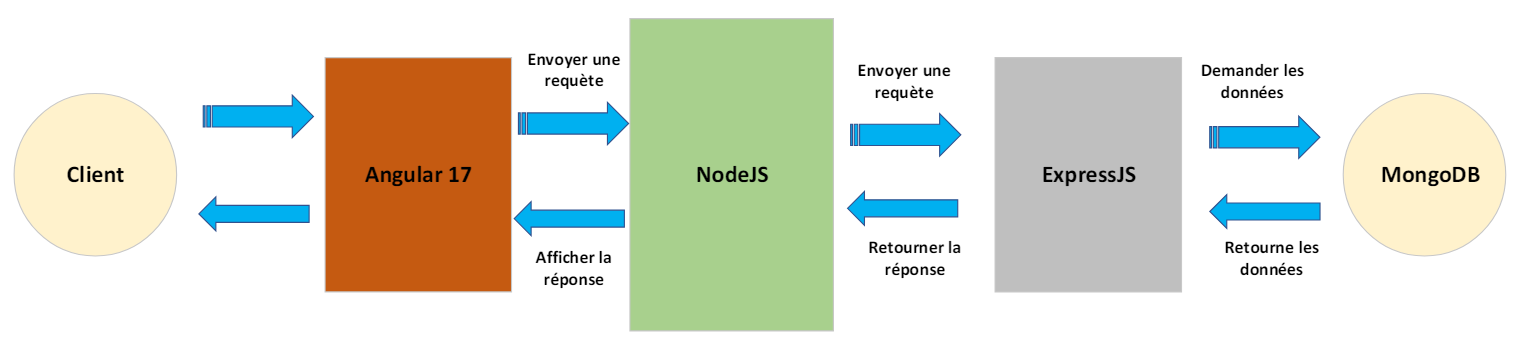
\includegraphics[width=0.5\columnwidth]{img/Architecture_MEAN.png}}
        \caption{Architecture MEAN }
        \label{fig:logo_tt}
    \end{figure}
    \subsection{Architecture adoptée.  } 
    Le MVC est un motif de conception (design pattern) qui sépare une application en trois composants logiques principaux : modèle, vue et contrôleur. Il propose une solution générale au problème de la structuration d’une application comme le montre la figure 20. \\
    Dans notre projet, le choix de ce modèle est exigé par le framework front-end   Angular, et le framework back-end Node js \\
    Le fonctionnement du patron est illustrer à travers la figure suivante :
    \begin{figure}[H]
        \centering
        \frame{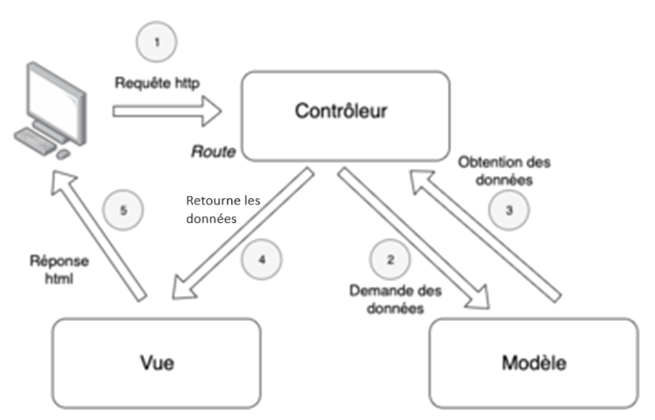
\includegraphics[width=0.5\columnwidth]{img/Architecture_MVC.png}}
        \caption{Architecture MEAN }
        \label{fig:logo_tt}
    \end{figure}
\section*{Conclusion}
Dans ce chapitre, nous avons préparé notre plan de travail. Nous avons présenté les besoins fonctionnels et non fonctionnels, les tâches des acteurs, le product backlog ainsi que la planification de la release, l'environnement de travail, et l'architecture et les patrons de conception. Dans le chapitre suivant, nous allons présenter le sprint 1 